
\documentclass[12pt,a4paper]{article}
\usepackage[utf8]{inputenc}
\usepackage{amsmath,amssymb,graphicx}
\usepackage{geometry}
\usepackage{hyperref}
\geometry{a4paper, margin=1in}

% Title and Author
\title{\textbf{Gerçek Hayat Mühendislik Problemlerinin Immune Plasma Algoritması ile Çözümü}}
\author{Fırat Kaan Bitmez - 23281855}
\date{2024-2025 Eğitim Öğretim Yılı Güz Yarıyılı}

\begin{document}

\maketitle

\section*{T.C. Ondokuz Mayıs Üniversitesi}
\subsection*{Lisansüstü Eğitim Enstitüsü}
\subsection*{Bilgisayar Mühendisliği}

\section*{Algoritma Tasarımı ve Karmaşıklık Analizi-BM631}
\vspace{0.5cm}

\begin{center}
\textbf{Gerçek Hayat Mühendislik Problemlerinin Immune Plasma Algoritması ile Çözümü}
\end{center}

\vspace{0.5cm}
\begin{flushright}
Fırat Kaan Bitmez - 23281855\\
SAMSUN, 2024-2025 Eğitim Öğretim Yılı Güz Yarıyılı
\end{flushright}

\section{Giriş}
Bu rapor, gerçek hayat mühendislik problemlerinden biri olan basınçlı kap tasarım probleminin Immune Plasma Algorithm (IPA) kullanılarak çözülmesini ele almaktadır. Basınçlı kap tasarımı, kimya, enerji, petrol ve gaz gibi birçok kritik endüstride karşılaşılan temel sorunlardan biridir. Bu problem, hem maliyet optimizasyonu hem de dayanıklılık açısından büyük önem taşır. Optimum bir çözüm, endüstriyel maliyetleri azaltmakla kalmaz, aynı zamanda üretim süreçlerini daha güvenli ve verimli hale getirir. Bu bağlamda IPA'nın uygulanabilirliği ve başarısı, mühendislik dünyasında yenilikçi bir çözüm olarak değerlendirilmektedir. IPA, biyolojik bağışıklık sistemlerinden ilham alınarak geliştirilmiş bir meta-sezgisel algoritma olup, mühendislik optimizasyon problemlerine çözüm sağlama kapasitesiyle dikkat çekmektedir.
IPA algoritmasının temel prensipleri, uygulama alanları ve algoritmanın özellikleri bu çalışmanın odak noktasını oluşturmaktadır. Rapor, algoritmanın uyarlanması, uygulama aşamaları, deneysel sonuçları ve literatürdeki diğer yaklaşımlarla karşılaştırılmasını kapsamaktadır.
Çalışmanın temel hedefi, Immune Plasma Algorithm'in performansının değerlendirilmesi ve bu algoritmanın çözüm süresinin, çözüm kalitesinin ve kıyaslamalarının detaylandırılmasıdır. Literatürde sıkça yer alan diğer algoritmalara kıyasla daha hızlı ve maliyet etkin bir çözüm sunup sunmadığını ortaya koymak bu çalışmanın önemli bir amacıdır.


\section{Problem Tanımı}
\subsection{Basınçlı Kap Tasarım Problemi}
Basınçlı kap tasarımı, mühendislik kısıtlamalarını karşılayan ve aynı zamanda malzeme ve üretim maliyetlerini optimize eden kritik bir optimizasyon problemidir. Bu süreçte, tasarım parametrelerinin maliyet üzerindeki etkisi ve kısıtlamaların ihlal edilip edilmediği matematiksel olarak değerlendirilir. Parametrelerin belirli sınırlar içinde değişim gösterdiği çözüm uzayı, maliyet fonksiyonunun minimize edilmesini ve geometrik ile fiziksel gereksinimlerin sağlanmasını mümkün kılar.

Amaç Fonksiyonu:
Bu problemde amaç fonksiyonu, maliyet ve dayanıklılık açısından optimum bir tasarım elde etmeye yönelik olarak tasarım parametrelerini optimize eder. Fonksiyon şu şekilde ifade edilir:

f(x)=0.6224x1x3x4+1.7781x2x32+3.1661x12x4+19.84x12x3
\\

•	İlk terim: Kap kabuğunun malzeme maliyetini temsil eder.

•	İkinci terim: Kap kapağının malzeme maliyetiyle ilişkilidir.

•	Üçüncü terim: Et kalınlığına bağlı maliyetleri içerir.

•	Dördüncü terim: Yarı çap ve malzeme maliyeti arasındaki ilişkiyi ifade eder.
\\
Kısıtlar:

Basınçlı kap tasarımında kullanılan kısıtlar aşağıda verilmiştir:

•	g1(x)=−x1+0.0193x3≤ 0 (Kabuk kalınlığı sınırı)

•	g2(x)=−x3+0.00954x32≤ 0 (Yarı çap geometrik sınırı)

•	g3(x)=−πx32x4− 4/3πx33+1296000≤ 0 (Hacim sınırı)

•	g4(x)=x4−240≤ 0 (Kap uzunluğunun üst sınırı)


Bu kısıtlar, tasarımın mühendislik ve fiziksel gereksinimlere uygunluğunu sağlamak için gereklidir. Optimizasyon algoritması, çözüm sürecinde kısıtların ihlal edilip edilmediğini sürekli kontrol eder. İhlal durumunda, algoritma yeni bir çözüm arayışına yönelir.

\subsection{Kısıtlar ve Matematiksel Kontrol}
\begin{align*}
g_1(x) &= -x_1 + 0.0193x_3 \leq 0 & \text{(Kabuk kalınlığı sınırı)}\\
g_2(x) &= -x_3 + 0.00954x_3^2 \leq 0 & \text{(Yarı çap geometrik sınırı)}\\
g_3(x) &= -\pi x_3^2x_4 - \frac{4}{3}\pi x_3^3 + 1296000 \leq 0 & \text{(Hacim sınırı)}\\
g_4(x) &= x_4 - 240 \leq 0 & \text{(Kap uzunluğunun üst sınırı)}
\end{align*}

Çözüm Sürecindeki Rolü:

•	Kısıt 1: Kabuk kalınlığının yarıçapa bağlı minimum bir değeri garanti eder.

•	Kısıt 2: Yarı çapın fiziksel ve geometrik tutarlılığını sağlar.

•	Kısıt 3: Kap hacminin belirlenen sınırlar içinde olmasını kontrol eder.

•	Kısıt 4: Kap uzunluğunun maksimum değeri aşmasını önler.


•	Kısıtlar, tasarımın fiziksel uygunluğunu ve mühendislik gerekliliklerini sağlar.

•	Optimizasyon algoritması, kısıt ihlalleri durumunda çözüm uzayını yeniden değerlendirir ve yeni bir yönelime geçer.

•	Kısıtların matematiksel kontrolü, çözümün uygulanabilirliğini ve güvenilirliğini garanti altına alır.
\subsection{Problemin Mühendislik Açısından Önemi}
Basınçlı kaplar, kimya, enerji, petrol ve gaz endüstrilerinde yaygın bir şekilde kullanılmaktadır. Başarısız bir tasarım, ciddi ekonomik kayıplara, tehlikeli patlamalara veya çevresel felaketlere neden olabilir. Bu nedenle, tasarımların güvenlik standartlarına uygun ve maliyet etkin şekilde optimize edilmesi kritik öneme sahiptir. Problemin karmaşık yapısı, gelişmiş optimizasyon algoritmalarının kullanımını gerektirir ve güvenilir, etkin çözümler sunmayı zorunlu kılar.

\section{Immune Plasma Algorithm (IPA)}

Immune Plasma Algorithm (IPA), biyolojik bağışıklık sistemlerinden esinlenerek geliştirilmiş ve karmaşık optimizasyon problemlerine etkin çözümler sunabilen bir algoritmadır. IPA’nın ana hedefi, çözüm alanında optimum sonuca hızlı ve etkili bir şekilde ulaşmaktır.
\subsection{Genel Çalışma Prensibi}
IPA, biyolojik bağışıklık sistemi fonksiyonlarından esinlenilerek tasarlanmış bir meta-sezgisel algoritmadır. Bu algoritma, bağışıklık sisteminin enfeksiyonlarla mücadeledeki temel mekanizmalarını matematiksel bir modelle birleştirir. Özellikle, enfeksiyon yayılımı ve bağışıklık tepkisi süreçleri, çözüm uzayının keşfi ve çözüm kalitesinin iyileştirilmesi için optimize edilmiştir. Enfekte bireylerin rastgele mutasyonlarla çeşitliliği artırması, bağışıklık yanıtının güçlü bireyleri koruyarak popülasyon performansını artırması gibi adımlar matematiksel olarak türetilmiş ve uygulanmıştır. Bu şekilde, biyolojik bağışıklık sistemindeki bilgi aktarımı ve öğrenme mekanizmaları, algoritmanın optimizasyon süreçlerine uyarlanmıştır. 
Aşağıdaki temel aşamaları içerir:

1.	Popülasyon Başlatılması: Popülasyon rastgele bireylerden oluşturulur. Bu bireyler problemin çözüm uzayında belirli bir çeşitlilik sağlar.

2.	Enfeksiyon Yayılımı: Rastgele bireyler enfekte edilerek çözüm uzayında çeşitlilik artırılır. Bu aşama, yeni potansiyel çözüm noktalarının bulunmasına katkı sağlar.

3.	Bağışıklık Tepkisi: Daha iyi performans gösteren bireyler korunur. Bu bireylerin bilgisi, algoritmanın başarı oranını artırır.

4.	Konvalesan Tedavi: Donör bireylerden alınan bilgi zayıf bireylere aktarılarak genel performans artırılır. Bu aktarım, popülasyonun genel çözüm kalitesini yüksek tutar.

\subsection{IPA Parametreleri}


    •	Popülasyon Boyutu: 100 birey

•	Maksimum Değerlendirme Sayısı: 100.000

•	Donör ve Alıcı Sayısı: 1 birey

IPA algoritmasının bu parametreleri, optimizasyon problemlerindeki başarı oranını belirleyen önemli faktörlerdir.


\section{Uygulama}
\begin{figure}[h!]
    \centering
    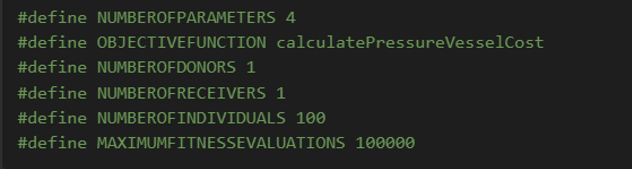
\includegraphics[width=0.5\linewidth]{1.png}
    \caption{IPA Algoritmasının Parametre Tanımlamaları}
    \label{fig:parameters}
\end{figure}

\subsection{IPA'nın Uyarlanması}
Immune Plasma Algorithm kaynak kodu şu parametrelerle ayarlanıp çalıştırılmıştır:
Kodun optimizasyonu sırasında, belirlenen parametreler algoritmanın matematiksel hesaplama süreçleriyle doğrudan ilişkilendirilmiştir. Özellikle:

•	NUMBEROFPARAMETERS: Problemin değişken sayısını belirler. Bu parametre, matematiksel modeldeki optimizasyon değişkenlerini ifade eder ve çözüm uzayının boyutunu kontrol eder.

•	LOWERBOUNDOFPARAMETERS ve UPPERBOUNDOFPARAMETERS: Değişkenlerin alt ve üst sınırlarını belirler. Bu sınırlar, mühendislik kısıtlamalarını sağlamak için kullanılır.

•	OBJECTIVEFUNCTION: Optimizasyon sırasında minimize edilen maliyet fonksiyonunu tanımlar. Bu fonksiyon, her bireyin performansını matematiksel olarak değerlendirmek için kullanılır.

•	NUMBEROFDONORS ve NUMBEROFRECEIVERS: Her iterasyonda bilgi aktarımı yapan ve alan birey sayısını kontrol eder. Bu, IPA algoritmasının biyolojik bağışıklık sistemini taklit eden mekanizmasını optimize eder.

•	MAXIMUMFITNESSEVALUATIONS: Algoritmanın durma kriterini belirler ve hesaplama yükünü kontrol eder.


Bu parametreler, hem algoritmanın çalışmasını optimize etmek hem de belirlenen problem için en iyi sonuçları sağlamak üzere dikkatlice ayarlanmıştır.

Figure 1 'de Amaç fonksiyonu, maliyet optimizasyonu sağlamak için özelleştirilmiştir:

\begin{itemize}
    \item \textbf{NUMBEROFPARAMETERS}: Problemin değişken sayısını belirler.
    \item \textbf{LOWERBOUNDOFPARAMETERS ve UPPERBOUNDOFPARAMETERS}: Değişkenlerin alt ve üst sınırlarını belirler.
\end{itemize}
Figure'2 de calculatePressureVesselCost fonksiyonu, amaç fonksiyonunu ifade etmekte ve belirli kısıtlar altında çözümün uygunluğunu değerlendirmektedir. Bu parametreler, problemin gerçek hayatta uygulanabilirliğini sağlar.
\begin{figure}[h!]
    \centering
    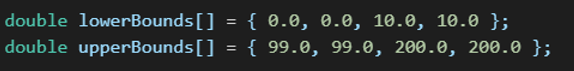
\includegraphics[width=0.5\linewidth]{2.png}
    \caption{Amaç Fonksiyonu ve Kısıtlar}
    \label{fig:objective}
\end{figure}

\subsection{MinGW Paketlerinin Yüklenmesi}
\begin{figure}[h!]
    \centering
    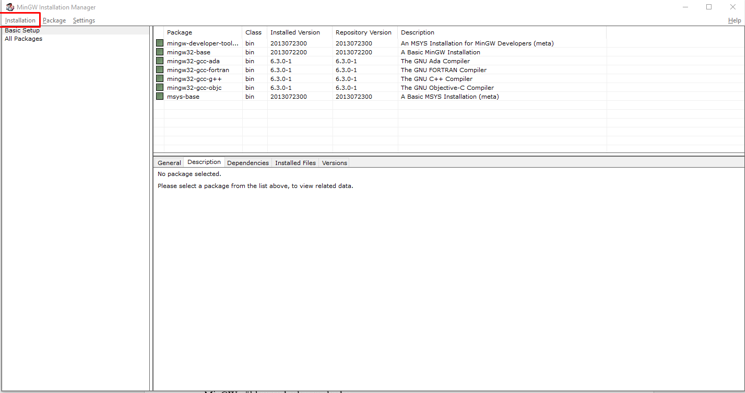
\includegraphics[width=0.5\linewidth]{3.png}
    \caption{MinGW Kurulum Ekranı}
    \label{fig:mingw}
\end{figure}
Algoritmayı çalıştırmak için MinGW ortamının doğru şekilde yapılandırılması gerekmektedir. MinGW yükleme adımları şunlardır:

1.	MinGW'nin resmi web sitesinden en son sürüm indirilir. https://sourceforge.net/projects/mingw/

2.	İndirilen kurulum dosyası çalıştırılarak yükleme başlatılır.

3.	"Basic Setup" sekmesi seçilir ve gerekli paketler işaretlenir:

o	mingw32-gcc-g++: C++ derleyicisi
o	mingw32-gcc-objc: Objective-C desteği
o	msys-base: Temel MSYS araçları
4.	İşaretlenen paketler kurulum listesine eklenir ve "Apply Changes" seçeneğiyle kurulum tamamlanır.

5.	Çevresel değişkenler (environment variables) ayarlanır:  
o	MinGW'nin kurulu olduğu dizin (ör. C:\MinGW\bin) PATH değişkenine eklenir.

6.	Kurulumun doğru yapıldığını doğrulamak için terminal veya komut istemcisine gcc --version komutu girilir.
\subsection{Deneysel Kurulum}
•	Donör Sayısı: 1 birey

•	Alıcı Sayısı: 1 birey

•	Popülasyon: 100 birey

•	Değerlendirme Sayısı: 100,000

\subsection{Deneysel Sonuçlar}
Kod, Dev-C++ derleyicisi kullanılarak çalıştırılmış ve şu sonuçlar elde edilmiştir:

•	En iyi maliyet: 37.54494

•	Geçen Süre: 0.053 saniye

Sonuçlar, algoritmanın hem maliyet hem de performans açısından etkinliğini göstermektedir.

\begin{figure}[h!]
    \centering
    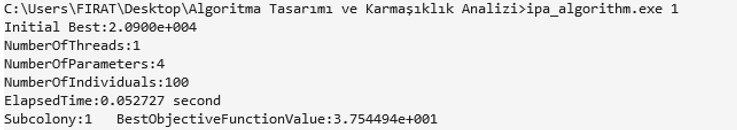
\includegraphics[width=0.5\linewidth]{4.png}
    \caption{Deneysel Sonuç Çıktıları}
    \label{fig:results}
\end{figure}

\section{Analiz ve Karşılaştırma}
Figure 5'de IPA algoritması, literatürdeki diğer meta-sezgisel algoritmalarla karşılaştırılmıştır. Bu karşılaştırmada, algoritmaların seçimi optimizasyon problemlerindeki yaygın kullanımları ve farklı problemlerdeki etkinlikleri göz önüne alınarak yapılmıştır. Genetic Algorithm (GA) ve Particle Swarm Optimization (PSO) gibi popüler algoritmalar, hem çözüm kalitesi hem de hesaplama verimliliği açısından karşılaştırma için uygun bulunmuştur. Bu algoritmalar, literatürdeki başarı oranları ve şu anki uygulamalarındaki yaygınlıkları nedeniyle tercih edilmiştir. Karşılaştırma kriterleri arasında çözüm maliyeti, algoritmanın çalışma süreci ve optimizasyon performansı yer almaktadır. Bu kriterler, endüstriyel uygulamalardaki çözüm gereksinimlerini karşılamada algoritmaların uygunluğunu değerlendirmek için temel ölçülerdir. İlgili algoritmalar ve performansları aşağıdaki gibidir:
\begin{figure}[h!]
    \centering
    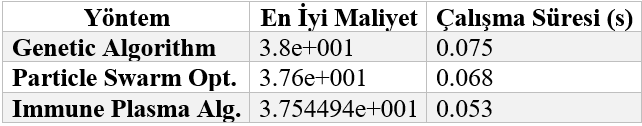
\includegraphics[width=0.5\linewidth]{5.png}
    \caption{Karşılaştırmalı Performans Tablosu}
    \label{fig:comparison}
\end{figure}


Tablodan görüldüğü üzere, IPA hem maliyet açısından daha iyi sonuçlar üretmiş hem de çalışma süresi açısından diğer yöntemlere kıyasla daha hızlıdır.

\section{Sonuçlar}
Bu çalışmada, Immune Plasma Algorithm kullanılarak basınçlı kap tasarımı probleminin başarıyla çözüldüğü gösterilmiştir. IPA, literatürdeki diğer algoritmalara kıyasla daha düşük maliyet ve daha hızlı çalışma süresi sunmuştur. Algoritmanın çözüm kalitesi, gerçek hayatta uygulanabilirliğini arttırmaktadır.
Gelecekte, IPA'nın farklı mühendislik problemlerinde kullanılabilirliğini ve performansını daha da artıracak parametre optimizasyonlarının çalışılması planlanmaktadır.

\section{Kaynaklar}
\begin{enumerate}
    \item Abualigah, L. (2022). Meta-heuristic Optimization Algorithms for Engineering Problems.
    \item Demirci, S. (2025). Immune Plasma Algorithm: A Novel Metaheuristic.
    \item Kaynak Kod: ImmunePlasmaAlgorithm\_Version1.c
\end{enumerate}

\end{document}
